\documentclass{ctexart}
\usepackage{graphicx}
\title{零钱找零:动态规划}
\author{Ngoo Ling Hui}
\begin{document}
\maketitle

\section{概述}
本报告旨在介绍对教学代码进行整理和重构的过程,以建立一个包含二叉搜索树、AVL树、红黑树和伸展树的统一架构。通过使用继承关系和虚类来表达它们之间的逻辑关系,并在一个名为 BinaryTree.h 的头文件中整合所有代码。

\section{整体设计思路}
本设计采用了面向对象的设计思想,使用继承关系将不同类型的二叉树归为一个树结构的整体。设计了一个基础虚类 BinaryTree 作为最顶层的基类,规范了所有二叉树的基本操作,如插入、删除和搜索。每个具体的二叉树类型(二叉搜索树、AVL树、红黑树和伸展树)都继承自 BinaryTree,并在需要的情况下重写了共同操作。

\section{代码结构}
\begin{enumerate}
    \item BinaryTree类:BinaryTree 类是所有二叉树操作的基类。它包含了通用的操作接口,如插入、删除和搜索,以及其他可能的共同操作。同时,它提供了中序遍历的实用函数。
    \item 具体二叉树类:
    \begin{itemize}
        \item BinarySearchTree 类:继承自 BinaryTree,实现了二叉搜索树的特定操作。
        \item AvlTree 类:继承自 BinarySearchTree,实现了AVL树的特定操作。
        \item RedBlackTree 类:继承自 BinarySearchTree,实现了红黑树的特定操作。
        \item SplayTree 类:继承自 BinarySearchTree,实现了伸展树的特定操作。
    \end{itemize}
    \item main 函数:在 TestTree.cpp 文件中编写了 main 函数,用于测试整合后的二叉树结构.
\end{enumerate}

\section{测试}
在 TestTree.cpp 中,编写了测试用例来验证整合后的二叉树结构的正确性。这些测试用例包括插入、删除、搜索等操作,以确保每个树类型都按预期工作。

\section{结论}
通过使用继承关系和虚类,成功地整合了不同类型的二叉树,并保留了它们的各自特定功能。这种设计使得代码更加模块化和可维护,提高了代码的可扩展性。报告中提供了对代码的整体设计思路和各部分功能的概述,以及测试的方法和结果。

\begin{figure}
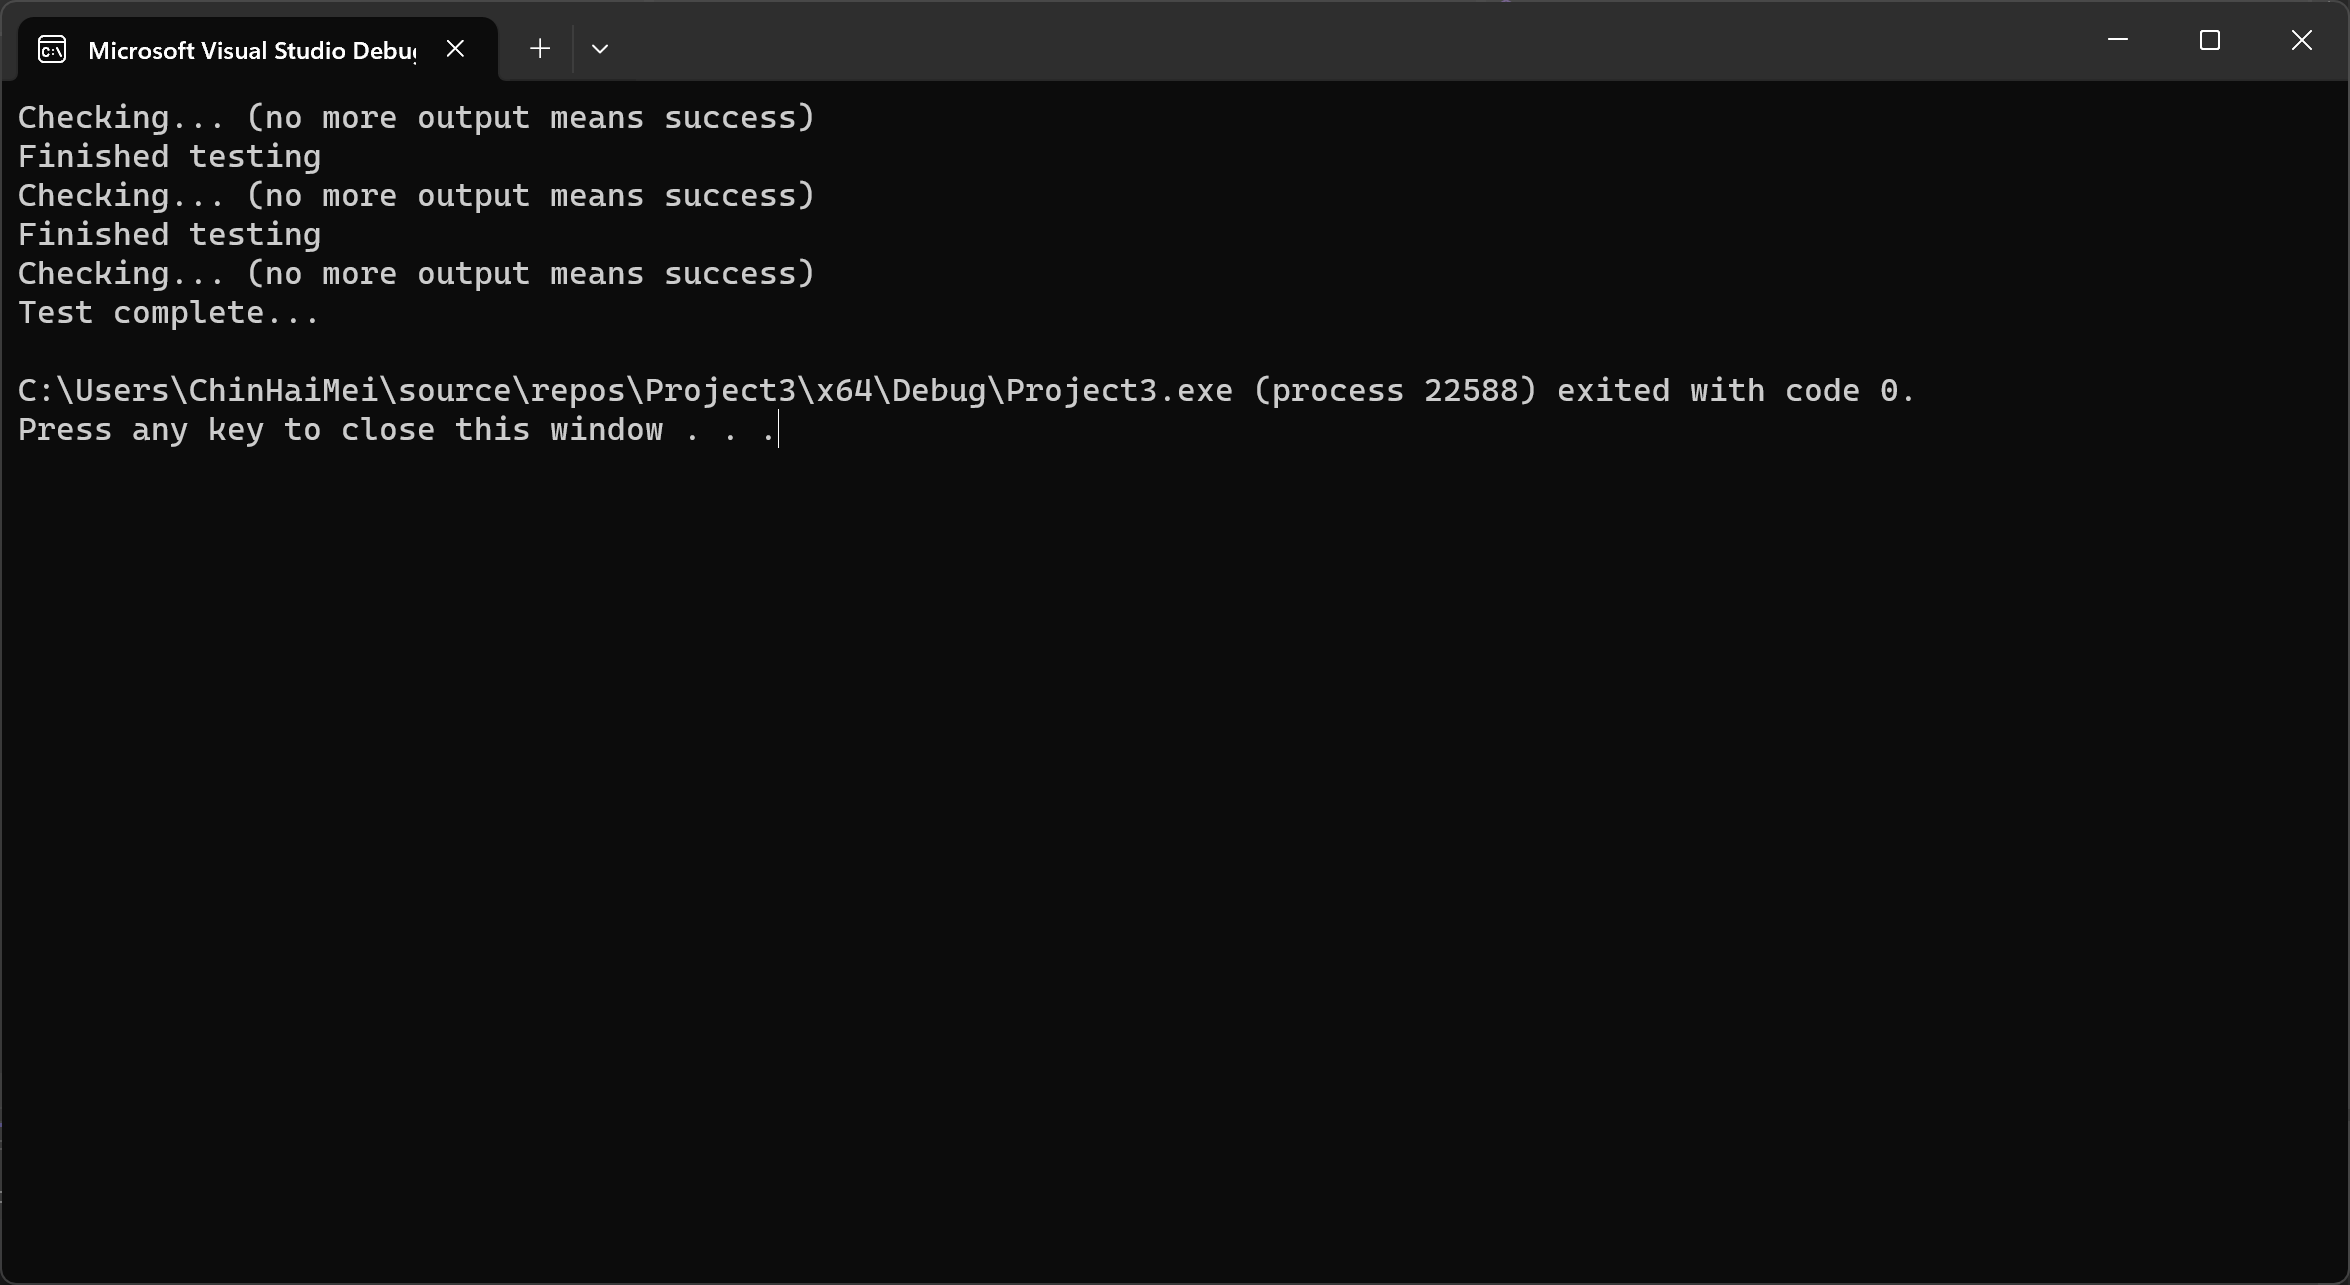
\includegraphics[width=0.5\textwidth]{image.png}
\end{figure}

\section{问题}
在整合的过程中,我遇到了一些关于Splay Tree的具体实现问题。尤其是在 `contains`,`findMin`,`findMax` 操作方面,我发现Splay Tree的实现方式与其他树存在const的差异。我尽最大努力完成Splay Tree的整合,但由于其特殊的行为,我可能无法完全符合其他树的标准接口。

尽管在本次整合中我未能完全解决Splay Tree的特殊问题,但我认为这是一个值得关注和改进的地方,可以在未来的工作中进一步探讨和优化。
    
\end{document}
